\section{NaCl framework}

The first part of my work for this thesis was the continuation of the development of a new framework designed to train spectrophotmetric models of type Ia supernova called NaCl ("Nouveaux Algorithmes de Courbes de Lumière") which was initially started by G. Augarde during his PhD, defended in September of 2022 (\cite{augar2022}).

In this section we will be defining the model that is trained by NaCl, this includes the parameterization of the model, the model constraints, regularization and error models. Finally we will be detailing how do we practically implement this into a code that can be used.

\subsection{The idea behind the framework}

The framework is meant to be able to easily train a spectrophotometric model all while being able to accurately propagate all know sources of uncertainties. It is meant to be easy to use and manipulate in order to account for any new developments in how spectrophotmetric models are parameterized. The idea is to then have a framework that is fast and capable of conducting model training easily every time one can do so on a cosmological dataset of type Ia supernova. We will see how this will allow us to overcome issues previous spectrophotometric models have encountered, such as calibration issues.

\subsection{Differences with the SALT models}


This parameterization is a classic principal component analysis, or PCA, with the addition of a color law. This presumes that the evolution of a supernova can be known with the help of 2 parameters : the stretch parameter $X_1$ and the excess color parameter $c$. The $M_0$ and $M_1$ surfaces along with the $CL$ color law are common to all supernovae. $M_0$ is the average spectral surface of a type Ia supernova, which represents what your average spectrophotometric evolution of a type Ia supernova looks like.
$M_1$ is a surface representing the main variations to $M_0$. $CL$ represents the color diversity of supernovae. It's also important to note that in NaCl we also determine the date of maximum emission of light $t_{max}$, which is hidden in the model parameters. Finally, in order to take into account the fact that the spectra aren't properly calibrated, we fit a third degree polynomial $SpecRecal(\lambda)$ for each spectra in the training dataset.\\

In practice we will be looking for $X_0$ as well so our spectral flux density will be written as $X_0 \times \mathcal{S}(\lambda,p)$. \\

To summarize, with the SALT2 parameterization, we are looking for global parameters that are $M_0$, $M_1$ and $CL$ common to all supernova and individual parameters $X_0$, $X_1$, $c$ and $t_{max}$ specific to each supernova. Determining the global parameters is what we called "training the model" while determining the individual supernova parameters is called "fitting the lightcurve parameters". In NaCl however, we are performing both at the same time and in this chapter they will be referenced together as "training" the model.


\subsubsection{Practical implementation of the SALT2 model}

In order to be able to determine the global model surfaces ($M_0$ and $M_1$), we will be describing them with the help of B-splines. This is a particular set of polynomials of order $m-1$, called splines of degree $m$, that can form a basis. Their smoothness will allow our model surfaces to have complex forms. We use splines of degree 4 in NaCl. $M_0$ and $M_1$ are then defined as :

\begin{equation}
    M_{0|1}=\sum_{k=1}^{n_p} \sum_{l=1}^{n_{\lambda}} \theta_{kl}^{[0|1]} \mathcal{B}_k(p) \mathcal{B}_l(\lambda)
    \label{eqn:model_spline}
\end{equation}

where $\mathcal{B}$ are the splines, $\theta$ are the model parameters that we will determine.\\

\noindent For the color law $CL(\lambda)$ it is implemented as a degree 5 polynomial. \\

\noindent The model parameters are then determined by minimizing a log-likelihood which takes the form of : 
\begin{equation}
    -2\ln(L) = N\ln(2\pi) + \ln(|\mathbf{V}|) + \mathbf{R}^T\mathbf{V}^{-1}\mathbf{R}
\end{equation}
where $\mathbf{R}$ are the model residuals and $\mathbf{V}$ the covariance matrix independent of the parameters. If $\mathbf{V}$ contains only measurement uncertainties, the problem then becomes minimizing the following quantity : 
\begin{equation}
    \chi^2 = \mathbf{R}^T\mathbf{V}^{-1}\mathbf{R}
\end{equation}
which will be the case for us during this PhD.

\subsection{Constraints}

Since this model is built empirically, we can see that there will be a lot of degeneracies between the individual and model parameters. To break those degeneracies we will be adding a set of constraints.\\ 

When NaCl was first developed, the constraints used were the same as the ones for SALT2 and SALT3 (\cite{Kenworthy_2021_SALT3}) models. 
Although those constraints break the degeneracies that exist between parameters, we've decided to include a new set of constraints that would address two things : the first that one of the constraints is non linear which made the model training take a longer time, the other was that some constraints depended on the supernovae used in the training sample. An example such a constraint was $<X_1> = 0$ which defined the average stretch of a supernovae. This is isn't an issue if we are comparing the stretch of supernovae that were fitted using the same model. However since NaCl will be used to train different models on different datasets, it'll be more difficult to directly compare the parameters of the supernovae.\\

During this PhD, the following sets of constraints were developed. I will be detailing what they do and why they were developed.\\

\noindent \textbf{\underline{\large{Model normalization:}}} \\


The model normalization is degenerated with the value of $X_0$. We impose that : 

\begin{align}
    \int M_0(\lambda,p=0)\frac{\lambda}{hc}B(\lambda)\mathrm{d}\lambda = 1 \label{eqn:M0norm}\\
    \int M_1(\lambda,p=0)\frac{\lambda}{hc}B(\lambda)\mathrm{d}\lambda = 0
\end{align}
where $B(\lambda)$ is the restframe standard $B$-band.\\


\noindent \textbf{\underline{\large{Date of maximum emission:}}} \\

There exists a degeneracy between the model and the date of maximum emission $t_{max}$. It’s possible to
shift the entire model in order to compensate for a change in the date $t_{max}$. For that we impose that at
$p = 0$, the model presents a maxima in the standard $B$-band :

\begin{align}
    \frac{\mathrm{d}}{\mathrm{d}p} \int M_0(\lambda,p=0)\frac{\lambda}{hc}B(\lambda)\mathrm{d}\lambda \Big{|}_{p=0} = 0 \\
    \frac{\mathrm{d}}{\mathrm{d}p} \int M_1(\lambda,p=0)\frac{\lambda}{hc}B(\lambda)\mathrm{d}\lambda \Big{|}_{p=0} = 0
\end{align}
\\

\noindent \textbf{\underline{\large{Color Law:}}} \\

We also need to account for the degeneracy that exists between the spectral shape of the model and $CL$. Tilting the $M_0$ and $M_1$ can be completely corrected for by changing $CL$. We impose then that $CL(B) = 0$ and $CL(V ) = 1$ with $B$ and $V$ being the central wavelengths of the restframe standard $B$-band and $V$-band.\\


\noindent \textbf{\underline{\large{Average color:}}} \\

Another degeneracy exists between the individual supernova color $c$ and the $M_0$. Changing the spectral features of the model can be completely compensated by the value of $c$. For that we need to define the "average" supernova color. 
We impose that the the $M_0$ surface would have its $B - V$ color equal to 0 at peak luminosity and that $c$ accounts for the relative variations in color with respect to that. The constraint now becomes :

\begin{equation}
    \int \left[ M_0(\lambda, p=0)B(\lambda) - M_0(\lambda, p=0)V(\lambda)   \right] \frac{\lambda}{hc} \mathrm{d}\lambda = 0
\end{equation}\\

\noindent \textbf{\underline{\large{Average stretch:}}} \\

A similar degeneracy also exists with $X_1$. A global change of the $X_1$’s can be absorbed by changing the shape of the $M_0$ surface along the phase axis. We have decided to fix the value of $X_1=1$ such that it would be equivalent to having the same $X_1$ value using SALT2. For that we fix the difference between the model evaluated for $X_1=0$ and $X_1 = 1$ at a phase of 15 :

\begin{equation}
    \int \left[M_0(\lambda, p=15) + M_1(\lambda, p=15) \right] \frac{\lambda}{hc}B(\lambda) \mathrm{d}\lambda - \alpha \int M_0(\lambda, p=15) \frac{\lambda}{hc}B(\lambda) \mathrm{d}\lambda = 0
\end{equation}
with $\alpha = 10^{-0.4 \times 0.162}$ the flux difference we have found in SALT2. \\

\noindent \textbf{\underline{\large{Average width:}}} \\

The last unwanted degree of freedom is regarding the width of the model. We can see that the definition of $X_1$ relies on a difference between the model with different stretch parameters but it doesn’t define what the width of the model is. We can always make the model larger or smaller while maintaining the constraints on all of the other parameters. One way to bypass that issue is to constrain the model at a certain phase. We choose to fix the model at a phase $p=15$, also known as $\Delta m_{15}$ as : 

\begin{equation}
    \int M_0(\lambda, p=15) \frac{\lambda}{hc} \mathrm{d}\lambda = 10^{-0.4}
\end{equation} \\

In practice, we write down the constraints as a function $C_k(\beta) = \alpha_k $ where $C_k(\beta)$ is a function evaluating the $k$-th constraint of value $\alpha_k$. This is then added as penalty that takes the form $\mu_{cons}\sum_k (C_k(\beta)-\alpha_k)^2$ where $\mu_{cons}$ is hyperparameter that determines the strength of the penalty. We can write this in a matrix $\mathbf{C}(\beta)$ and we obtain :

\begin{equation}
    \boxed{\chi_{cons}^2 = \mu_{cons} \mathbf{C}(\beta)^T \mathbf{C}(\beta)}
\end{equation}

\subsection{Regularization}

Because our training dataset contains a finite number of data points, it’s impossible that the entirety of the global parameters would be constrained by data. To deal with that we add regularization to the model during the fit, which is a penalty added to the model in the areas where we would have extremely large variations due to poor constraining power of the data. This is specifically really important for NaCl since we are fitting the date of maximum emission there are data points that could go outside of the model range. \\

The regularization penalty that was initially developed was expressed as :

\begin{equation}
    \mu_{reg} \sum_{kl} \left(  \theta_{k,l}^2 + \left( \theta_{k+1,l} - \theta_{k,l} \right)^2   \right)
    \label{eqn:old_reg}
\end{equation}

 where $\theta_{kl}$ are the model parameters as seen in equation \ref{eqn:model_spline}. The first sum is a penalty that makes the $\theta$'s tend to zero when no data is available. The second term is a penalty of the phase derivatives of the surfaces that limits the sharp variations of the model observed when no data is available, or at poorly constrained regions of the model. Finally, $\mu_{reg}$ is a hyperparameter that determines the strength of the penalty. Writing this in a matrix form gives us :

 \begin{equation}
     \chi^2_{reg} = \mu_{reg}\beta^T \mathbf{P} \beta
     \label{eqn:chi2_reg_old}
 \end{equation}
 where $\mathbf{P}$ is what we call the regularization matrix, that allows us to obtain the expression in equation \ref{eqn:old_reg}, and $\beta$ our set of parameters. \\
 An issue that we've had with this form of regularization is that it is very sensitive to the value of $\mu_{reg}$. If it's too small the model continues to present very strong variations. If it's too strong the model becomes attenuated and this biases our parameters, which means the cosmological parameters calculated with the output of NaCl would be biased. We show the effects of the strength of the regularization on the model in Figure \ref{fig:regularization} \\ 


 \begin{figure}[htpb]
\centering
\begin{subfigure}{0.9\textwidth}
    \centering
    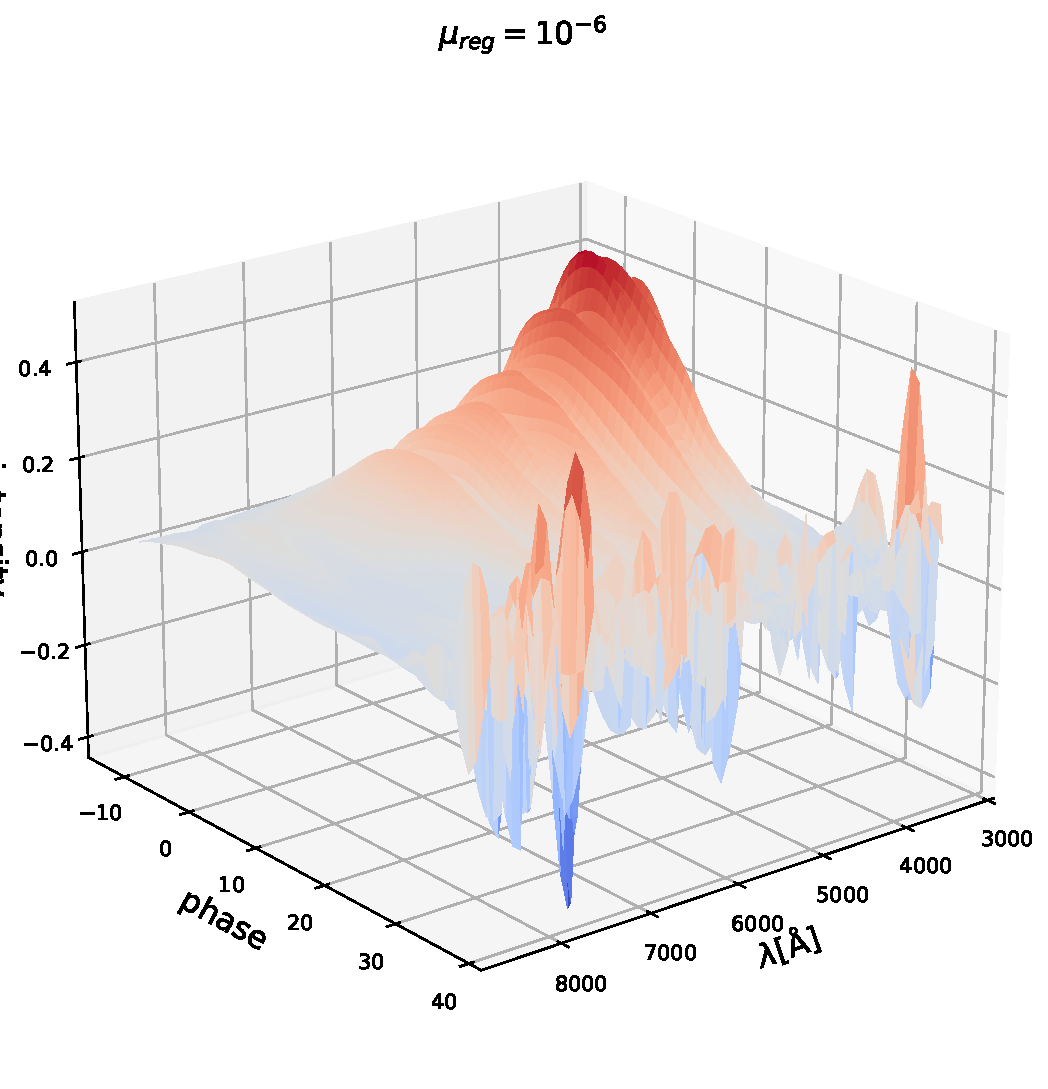
\includegraphics[width=.7\textwidth]{MainLayout/NaCl_chapter/figures/m0_e6_reg.pdf}
    \caption{}
    \label{fig:weak_reg}
\end{subfigure}%

\vspace{1em}

\begin{subfigure}{0.9\textwidth}
    \centering
    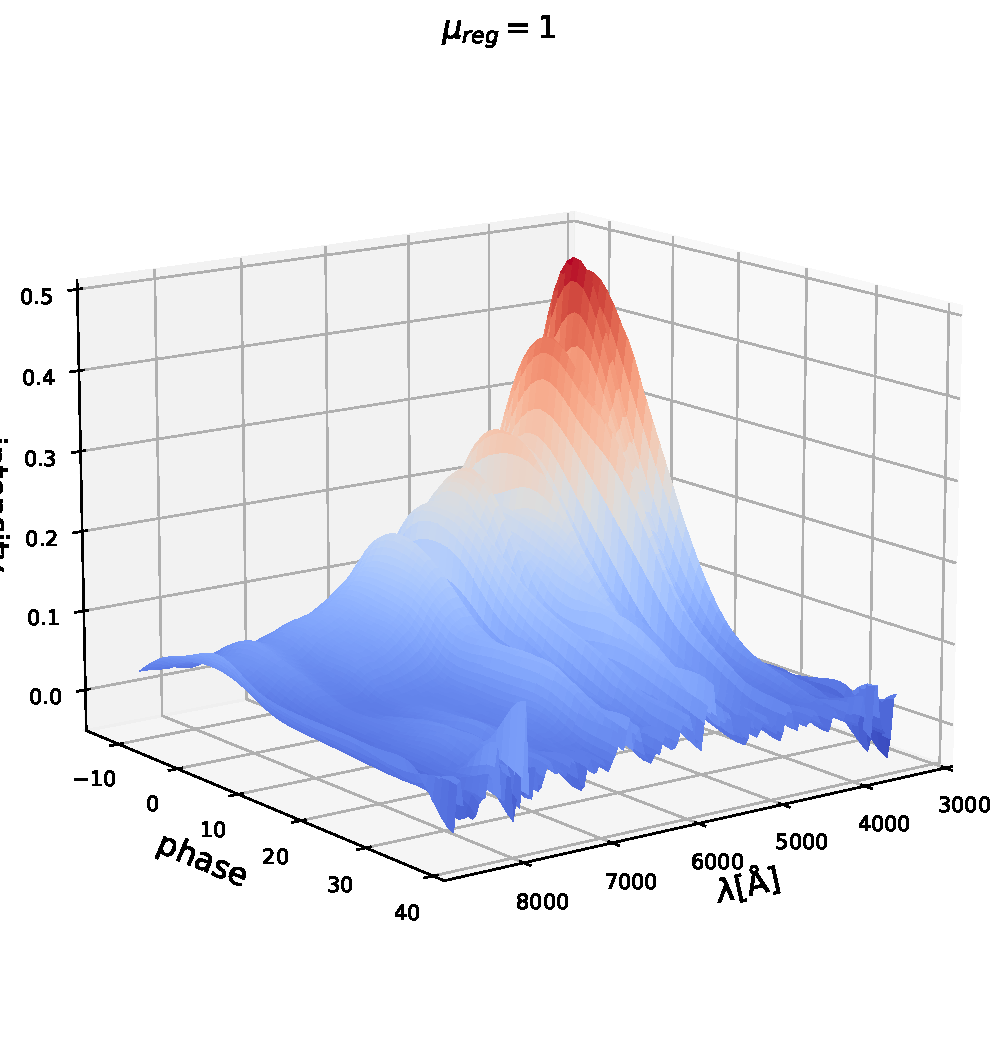
\includegraphics[width=.7\textwidth]{MainLayout/NaCl_chapter/figures/m0_e0_reg.pdf}
    \caption{}
    \label{fig:strong_reg}
\end{subfigure}
\caption{Effects of the strength of the regularization on the shape of the $M_0$. In \ref{fig:weak_reg} we see how the model behaves with a $\mu_{reg}=10^{-6}$. In \ref{fig:strong_reg} we see how the model behaves with a $\mu_{reg}=1$.}
\label{fig:regularization}
\end{figure}

To try and overcome this issue, I've developed during this PhD a regularization scheme that adapts the force of the regularization based on the number of points seen by each model parameter. This regularization scheme is inspired by \cite{lenz2022adaptiveregularizationbsplinemodels}. We can separate $\mathbf{P}$ matrix as follows : 

\begin{equation}
    \mathbf{P} = \mathbf{P}^{data} + \mathbf{P}^{smooth}
\end{equation}

with $\mathbf{P}^{data}$ and $\mathbf{P}^{smooth}$ the matrices determining the strength based on the number of points and to smoothen the model where there is no data as much as possible. In order to determine $\mathbf{P}^{data}$, we define $\mathcal{N}_i$ as the number of data points seen by each $\theta_{i}$ parameters ($\theta_{kl}$ written as a vector). We then introduce for each $\mathcal{N}_i$ a parameter $\mu_i$ which will act as a gate function of $\mathcal{N}_i$. This will determine the force of our regularization. The idea is that if $\mathcal{N}_i=0$ we regularize model strongly, otherwise we don't.\\

\textcolor{red}{COMMENT : This specific version of the regularization wasn't implemented in the final version of NaCl since we still had to test other things in between. I will be rewriting this part of the manuscript again.}

$\mu_i$ is then defined as : 

\begin{equation}
  \mu_i^{data} = \mathrm{max}(\mu_{reg}^{data} - \mathcal{N}_i, 0)
  \label{eqn:reg_mu}
\end{equation}

We can use that to define a diagonal matrix $\mathbf{M}^{data}$ where $\mathbf{M}_{ii}^{data} = \mu_i^{data}$. It is then clear that the simplest way to define $\mathbf{P}^{data}$ will be to write it as :

\begin{equation}
    \mathbf{P}^{data} = \mathbf{M}^{data} \times \mathbb{1}
\end{equation}

\noindent We then define $\mathbf{P}^{smooth}$ as a penalty on the first order derivative of the model in phase, like in equation \ref{eqn:old_reg}. We apply the same adaptive method mentioned previously and we get :

\begin{equation}
    \mathbf{P}^{smooth} = \mathbf{M}^{smooth} \times \mathbb{P}
\end{equation}

with $\mathbb{P}$ being : 
\begin{equation}
     \mathbb{P} = \begin{bmatrix} 
     2  & -1& 0  &   &     &...  \\
     -1 & 1 & -1 & 0 & ... & \\  
     0  &   &    &...&     &  \\  
        &   &... &   &     &  0\\ 
        &...& 0  & -1& 1   & -1 \\  
     ...&   &    & 0 & -1  & 2 \end{bmatrix}
\end{equation}
with $\mu_{reg}^{smooth}$ would be the hyperparameter determining the strength of the regularization on the derivatives.\\
Since the hyperparameters are now included in the  $\mathbf{P}$ matrix, the penalty now becomes : 
\begin{equation}
     \boxed{\chi^2_{reg} = \beta^T \mathbf{P} \beta}
     \label{eqn:chi2_reg_new}
 \end{equation}

\subsection{Error models}

Dealing with an empirical model means that we expect that our model would not perfectly describe the data. More specifically, the residuals of the model would not be explained solely by the measurement uncertainties on the data. This is a variability that exists between supernovae, unable to be captured by the SALT2 parameterization.\\
It's also important to note that all of the photometric measurements are affected by uncertainties of the photometric instruments. This can play a crucial role in our measurements of cosmological parameters as it has been shown in the most recent analyses to be one of the leading systematics (\cite{rubin2024unionunitycosmology2000}, \cite{vincenzi2024darkenergysurveysupernova}).\\
We can account for both the supernova variability and calibration uncertainties with the help of error models.\\

\subsubsection{Error Snake}

The first error model is the Error Snake, which is supposed to capture errors directly due to variability in the flux. If we call $V$ the variance of the data points, then the error model is implemented as :
\begin{equation}
    V = \sigma_{meas}^2 + \sigma_{snake}^2
\end{equation}
where $\sigma_{meas}$ are the measurement uncertainties and $ \sigma_{snake}$ is the additional variance added that is our Error snake model.\\

The general expression of this term is :
\begin{equation}
    \sigma_{snake} = G(\lambda, p) \times \phi(\lambda,p)
\end{equation}
where $\phi$ is the concatenation of both the measured photometric and spectroscopic fluxes used in our training dataset. $G(\lambda, p)$ can take multiple forms depending on how we would like to model our Error snake. \\

The simplest way to model it would be as a constant. The expression becomes : 
\begin{equation}
    G(\lambda, p) = g
\end{equation}
Physically this means that the variability of the supernovae in our dataset are independent of phase and wavelength.\\

Alternatively, we can imagine something more complex by modeling $G$ as a surface like $M_0$ and $M_1$ that is to be determined during the training. The expression then becomes:
\begin{equation}
    G(\lambda, p) = g(\lambda, p)
\end{equation}
Here, the variability does depend on phase and wavelength.\\

Lastly, we thought of adding a bit more complexity in our Error snake since we know that it's possible that our dataset could be contaminated by very peculiar supernovae or by objects that are hard to distinguish from type Ia supernova such as type Ib and type Ic supernovae or . We decided to also include an extra term in $G$ that takes up one value for each supernova in our dataset, we call it $\gamma_{SN}$. We expect that the $\gamma_{SN}$ value of a peculiar supernova would be larger than the others. The expression then becomes : 

\begin{equation}
    G(\lambda, p) = \gamma_{SN} \times g(\lambda, p)
\end{equation}

which is what we would like to use in the final analysis of the LEMAÎTRE dataset. However it is important to note that for the data challenges, specifically DC1 (see Chapter 4), we will be using the simplest form of the Error snake.

\begin{figure}[htpb]
\centering
\begin{subfigure}{1\textwidth}
    \centering
    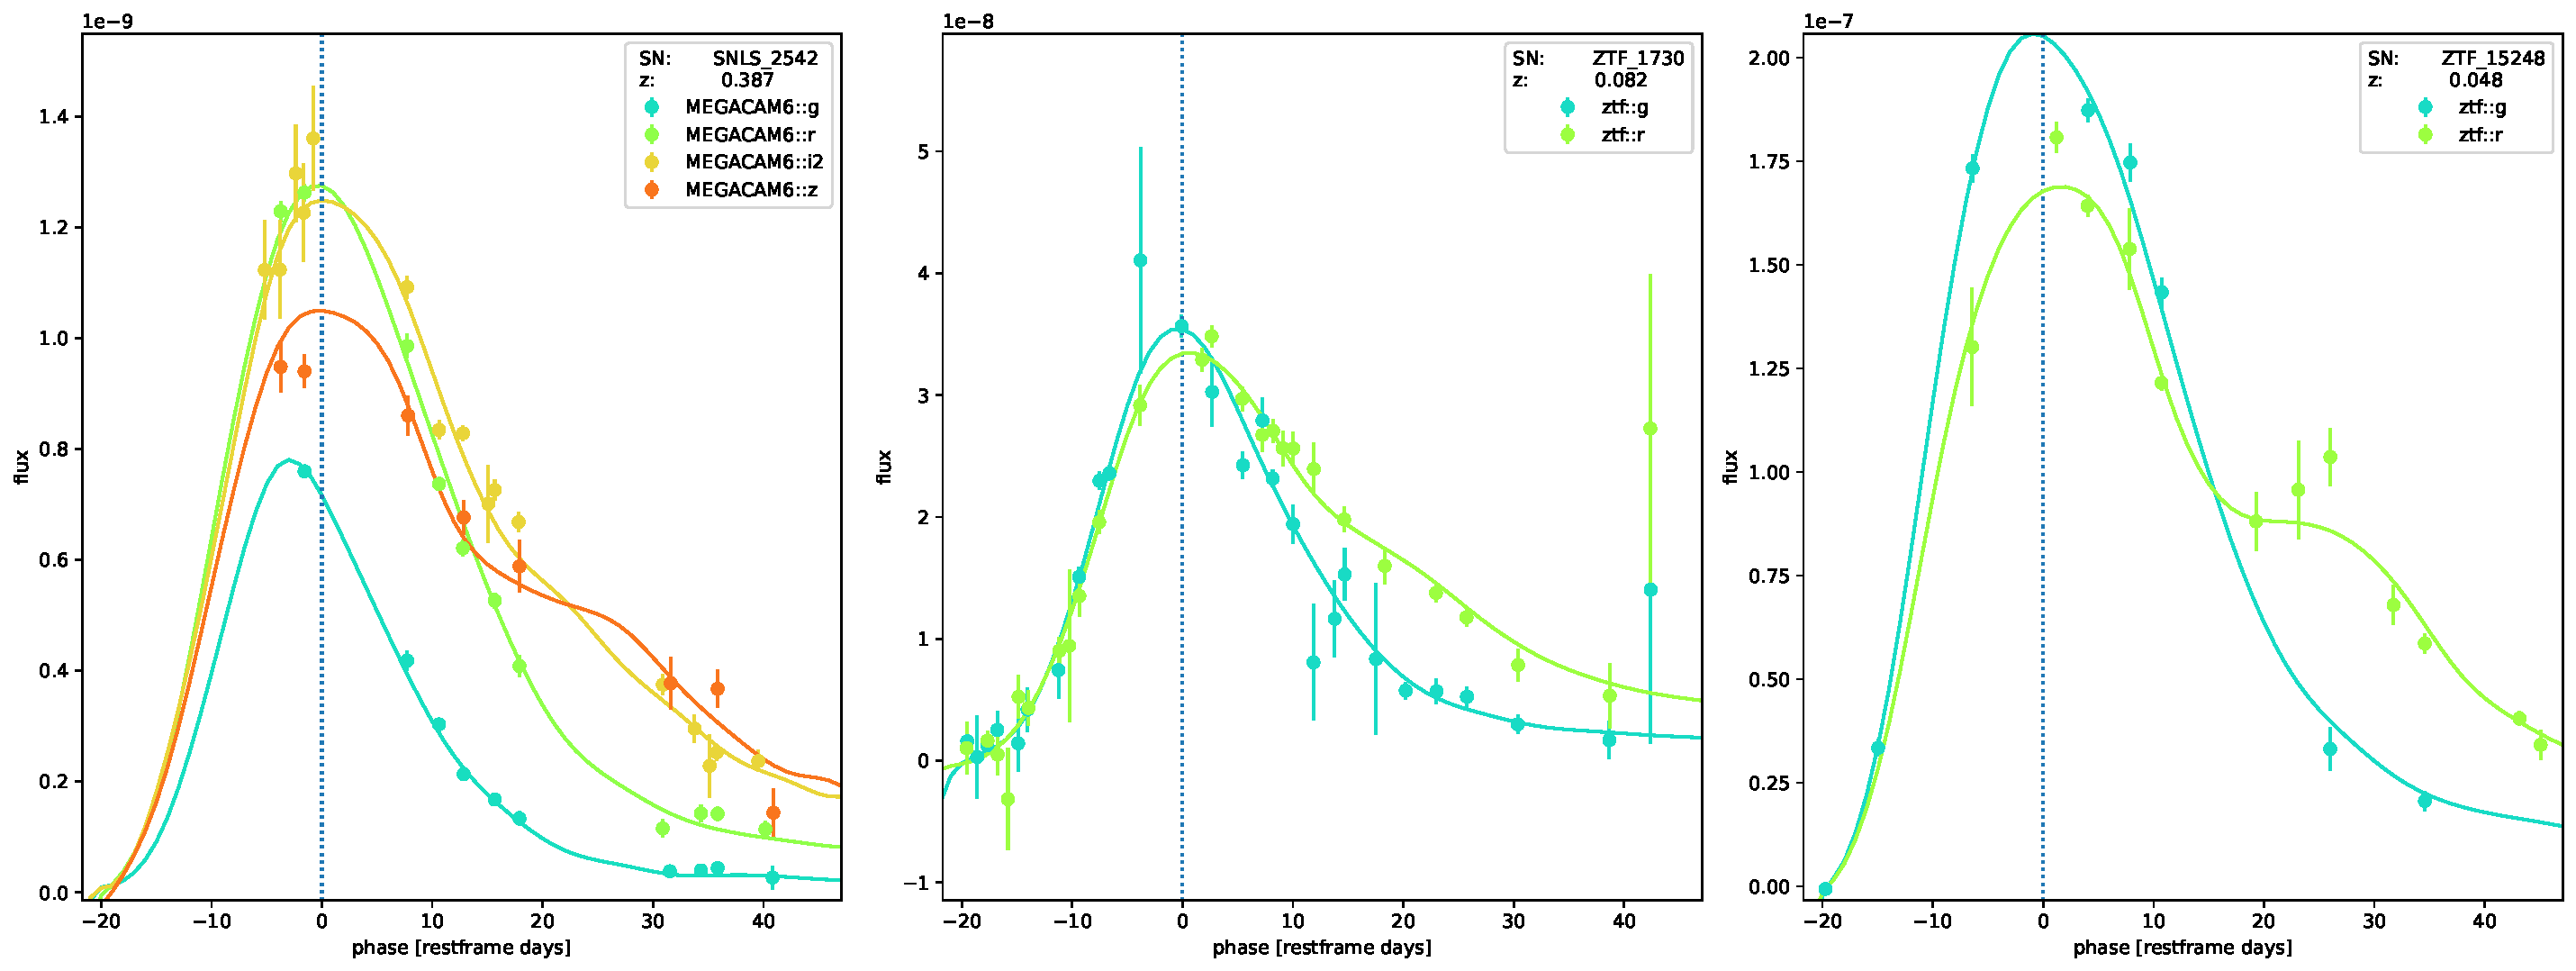
\includegraphics[width=1.1\textwidth]{MainLayout/NaCl_chapter/figures/lcs_without_snake.pdf}
    \caption{}
    \label{fig:nosnake}
\end{subfigure}%

\vspace{1em}

\begin{subfigure}{1\textwidth}
    \centering
    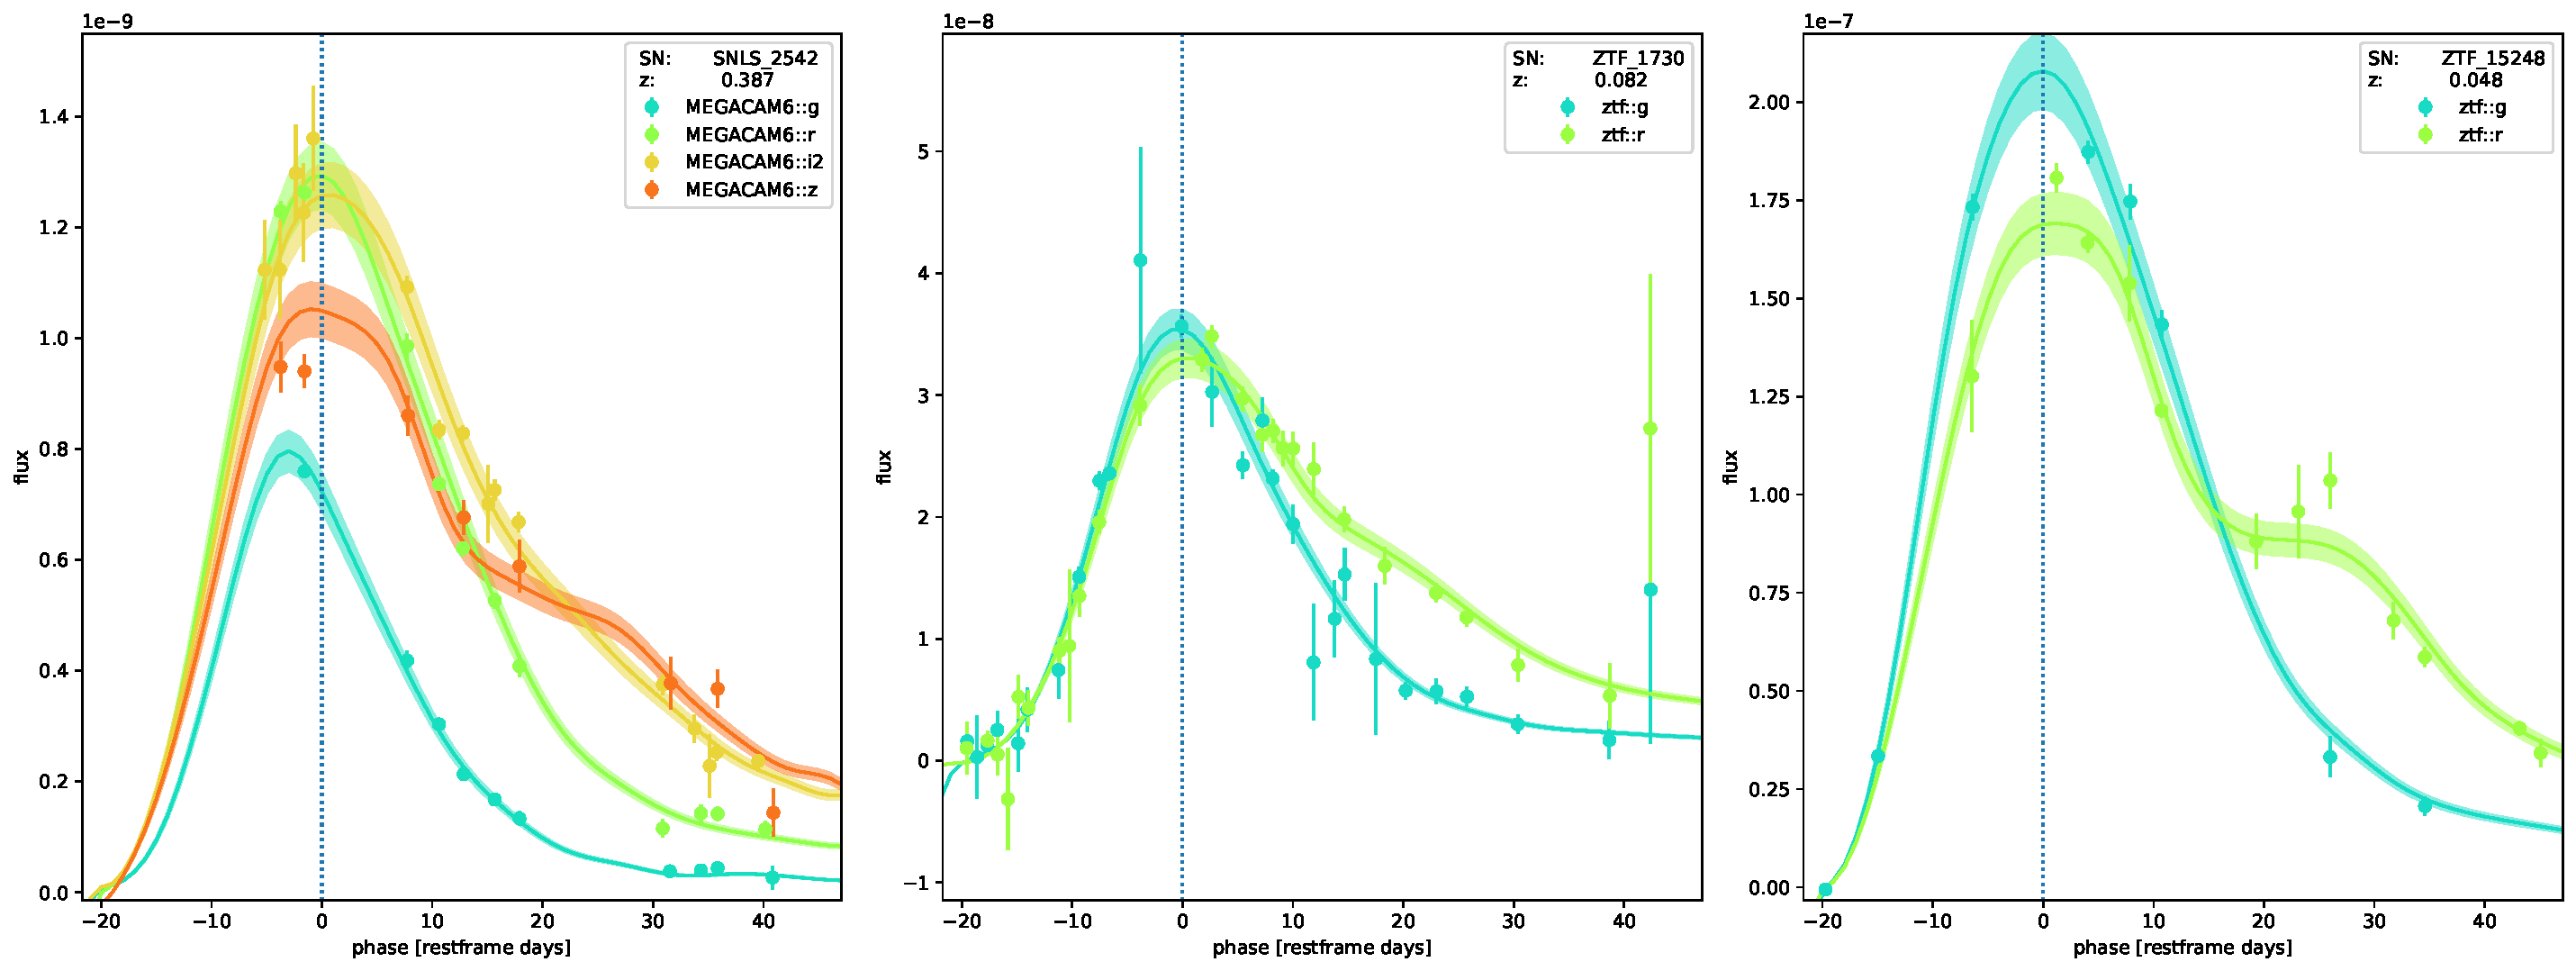
\includegraphics[width=1.1\textwidth]{MainLayout/NaCl_chapter/figures/lcs_with_snake.pdf}
    \caption{}
    \label{fig:snake}
\end{subfigure}
\caption{Visual representation of the error snake on simulated lightcurves from DC1 (see section (reference)). In \ref{fig:nosnake} we see how the model represents the data without an error snake model. In \ref{fig:snake} we see a highlighted section for each lightcurves which are the variations modeled by the error snake.}
\label{fig:errorsnake}
\end{figure}

\subsubsection{Color Scatter}

\noindent \textcolor{red}{COMMENT : Waiting for the final implementation}

\subsubsection{Calibration Uncertainties}

The calibration uncertainties are taken into account directly in the model. One parameter $\eta$ is added for each transmission band in our dataset held by a prior that is known beforehand. For the LEMAÎTRE project we have 12 bands, so we'll have 12 $\eta$ parameters. The expression of the photometric model becomes : 

\begin{equation}
    \phi_{phot}(\lambda, p) = X_0 (1+\eta) (1+z) \int S(\lambda, p) T(\lambda) \frac{\lambda}{hc}\mathrm{d}\lambda
\end{equation}

With an additional penalty to the model :

\begin{equation}
    \chi^2_{calib} = \mathbf{\eta}^T \mathbf{V_{\eta}}^{-1}\eta
\end{equation}
$\mathbf{V_{\eta}}$ being the $\eta$ covariance matrix that is already known.


\subsection{NaCl output}

At the end of a training, we get a vector containing all of the model and individual supernova parameters and the full covariance
 matrix calculated from the Hessian of the model : $  \mathbf{V} = 2 \mathbf{H}^{-1}$. For the cosmological analysis, we will be marginalizing 
 over all but the $X_0$, $X_1$ and $c$ parameters. \\

\begin{figure}[ht]
    \centering
    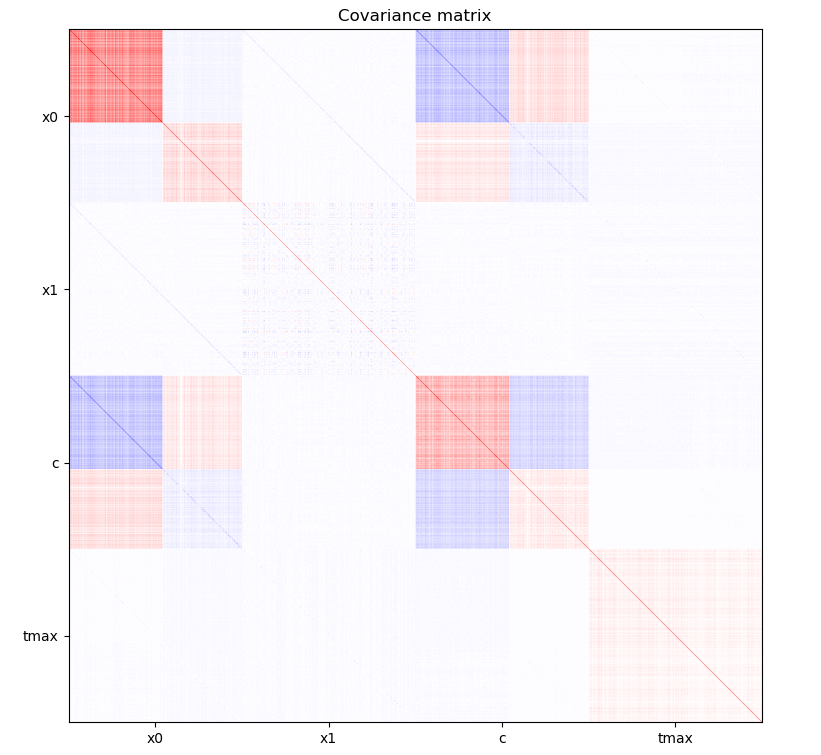
\includegraphics[width=1.0\textwidth]{MainLayout/NaCl_chapter/figures/covariance matrix.png}
    \caption{Example of the NaCl covariance matrix after an output, marginalized over all but the $X_0$, $X_1$ and $c$ parameters.}
    \label{fig:corr_mat_nacl}
\end{figure}